\documentclass[border=8pt]{standalone}
\usepackage{amsmath}
\usepackage{amssymb}
\usepackage{fontspec}
\setmainfont{Source Serif 4}
\usepackage{tikz}
\usetikzlibrary{positioning, arrows.meta}
\definecolor{qbase}{RGB}{31,86,160}

\begin{document}
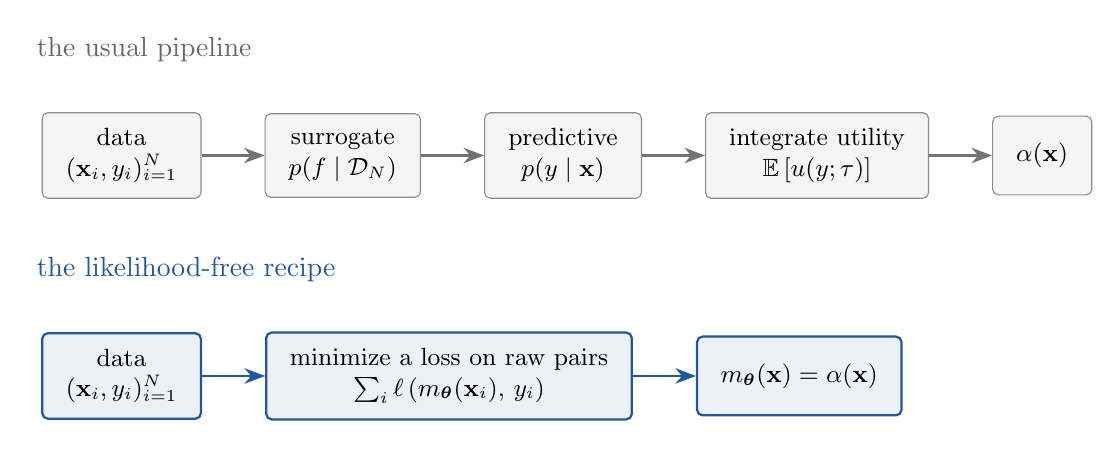
\begin{tikzpicture}[
  font=\small,
  box/.style={draw, rounded corners=2pt, minimum height=10mm, inner xsep=3mm,
              inner ysep=2mm, align=center},
  gbox/.style={box, draw=black!45, fill=black!4},
  bbox/.style={box, draw=qbase, fill=qbase!8, thick},
  garr/.style={-{Stealth[length=2.6mm]}, black!55, thick},
  barr/.style={-{Stealth[length=2.6mm]}, qbase, thick},
]
\node[font=\normalsize, black!60, anchor=west] at (-0.2, 1.35) {the usual pipeline};
\node[gbox] (d1) at (1.0, 0) {data\\ $(\mathbf{x}_i, y_i)_{i=1}^{N}$};
\node[gbox, right=8mm of d1] (post) {surrogate\\ $p(f \mid \mathcal{D}_N)$};
\node[gbox, right=8mm of post] (pred) {predictive\\ $p(y \mid \mathbf{x})$};
\node[gbox, right=8mm of pred] (integ) {integrate utility\\ $\mathbb{E}\left[ u(y; \tau) \right]$};
\node[gbox, right=8mm of integ] (a1) {$\alpha(\mathbf{x})$};
\draw[garr] (d1) -- (post);
\draw[garr] (post) -- (pred);
\draw[garr] (pred) -- (integ);
\draw[garr] (integ) -- (a1);

\node[font=\normalsize, qbase, anchor=west] at (-0.2, -1.45) {the likelihood-free recipe};
\node[bbox] (d2) at (1.0, -2.8) {data\\ $(\mathbf{x}_i, y_i)_{i=1}^{N}$};
\node[bbox, right=8mm of d2] (loss) {minimize a loss on raw pairs\\ $\sum_i \ell\left( m_{\boldsymbol{\theta}}(\mathbf{x}_i),\, y_i \right)$};
\node[bbox, right=8mm of loss] (a2) {$m_{\boldsymbol{\theta}}(\mathbf{x}) = \alpha(\mathbf{x})$};
\draw[barr] (d2) -- (loss);
\draw[barr] (loss) -- (a2);
\end{tikzpicture}
\end{document}
